\documentclass[10pt]{jreport}
\usepackage{./grad}
\usepackage[dvipdfmx]{graphicx}
\usepackage{here}
\usepackage{url}
\usepackage{bm}
\usepackage{amsmath}
\usepackage{comment}



\title{VANETにおける車両位置とリンク状態を考慮した地理的
opportunistic routing}
\vspace{4cm}
\author{%
高橋 柊人\\
立命館大学\\
情報理工学部\\
情報コミュニケーション学科 4回生\\
学籍番号 : 2600160225-9\\
指導教員 : 野口 拓, Alberto Gallegos Ramonet\\
2019年度(秋学期)卒業研究3(2B)\\
}
\date{令和4年1月31日}

%\renewcommand{\baselinestretch}{2.0}

\begin{document}

\maketitle

\renewcommand{\thepage}{\roman{page}}
\setcounter{page}{1}
\addcontentsline{toc}{chapter}{内容梗概}
\chapter*{内容梗概}
本論文は,筆者が立命館大学情報理工学部において行った「VANETにおける車両位置とリンク状態を考慮した地理的
opportunistic routing」の成果をまとめたものである.

近年, 高速道路や一般道での無謀な運転や不注意運転による交通事故が問題となっている. 交通死亡事故の原因の中では, 規制速度を超過した場合の割合が3割を占めることがわかっている. また, 交通事故死亡者数と取り締まり件数に注目すると, 取り締まりが増加すると死者数が減少するデータもある. これらのことから, 交通事故の死亡者数を減らすためには, より多くの速度超過の監視が求められる.

一方, 近年無線通信機器を搭載した車両間のみでネットワークを構築するVANET(VehicularAd-Hoc Network)に関する研究が盛んに行われている. VANETの利用方法の一つとして, 速度超過の監視が期待される. しかし、VANETの通信の基本手法であるフラッディングは, 車両密度が高くなると, 大量のパケットが一度にネットワーク内にブロードキャストされ, 冗長なパケットの発生やパケットの衝突が発生する問題が存在する.

そこで本論文では, 高速道路を想定したシナリオで, VANETを用いて速度超過車両の検出するための速度推定手法とブロードキャスト制御手法を提案した. 提案手法では, 速度超過を行う可能性のある車両情報のみのブロードキャストを行い, さらにブロードキャストを受信した車両それぞれが位置情報を用いて待ち時間を設定することによって, 冗長な情報を再ブロードキャストする車両台数の削減を行った.

性能評価では, ブロードキャストの回数, 再ブロードキャストの削減率, 速度超過車両の検出確率の検証を行った. シミュレーションによる実験の結果, 提案手法が既存手法に比べてブロードキャストを大幅に削減し, 速度超過車両の検出確率を同様に保つことができた.


\newpage
\pagestyle{myheadings}
\renewcommand{\thepage}{\roman{page}}
%\setcounter{page}{1}
\addcontentsline{toc}{chapter}{目次}
%\setcounter{page}{1}
\tableofcontents

\newpage
\renewcommand{\thepage}{\arabic{page}}
\setcounter{page}{1}
\chapter{緒論}
\vspace{-5mm}
高速道路や一般道での無謀な運転や不注意運転によるほかのドライバへの危険が問題となっている. もし, これらの危険行為を行う車両の接近を遭遇する以前に知ることができれば, 多くの事故を減らすことができる可能性がある. 交通死亡事故の原因の中では, 規制速度を超過した場合の割合が31.6%\cite{1}と, 速度違反が死亡事故につながることがわかる. また, 交通事故死亡者数と取り締まり件数に注目すると, 取り締まりが増加すると死者数が減少するデータもある. これらのことから, 交通事故の死亡者数を減らすためには, より多くの速度超過の監視が求められる. 
 
現在, 多くの道路では, カメラや速度センサを用いた速度違反車両の監視を行っている. しかし, この方法には観測地点以外の場所で検知されずに速度超過を行うことができる欠点が存在する. さらには, 近年このような監視を行うカメラやセンサが付近にあることを知らせるシステムも存在する\cite{sample2}. 
 
一方, 近年, 無線通信技術の発展により, 無線LANや, モバイルアドホックネットワーク, 無線センサネットワークなど様々な研究がされている. その中で, 通信に基地局や無線LANアクセスポイントを必要とせず, 端末のみで通信ネットワークを構成するモバイルアドホックネットワーク(MANET)が注目を浴びている. MANETの有望な利用方法の一つとして車両アドホックネットワーク(VANET)\cite{sample3}があげられる. VANETは車両がノードとなりネットワークを構成し, 固定インフラに頼らず車両間で情報交換が可能である. VANETを用いたアプリケーションとして, 渋滞回避情報や緊急車両走行情報の共有, 車両同士の衝突防止を目指した安全運転支援などが期待されている\cite{sample4}\cite{sample5}. また, 車載のレーダーやカメラなどの無線通信機器によって通信する場合, 専用の無線通信機器を車両に搭載しなければならない. VANETの性質上, 自車両以外の車両にも無線通信機器が搭載されていなければ, 成立しないため多くの車両に通信機器が搭載されることで初めて真価を発揮すると言える. そのため現状では, 通信機器の普及やコストが問題として挙げられる. また, VANETでは情報を車両がブロードキャストで中継し, マルチホップ通信を行うことで通信可能な範囲に存在するすべての車両に情報を配信することが可能である. しかし, 車両密度が高い地域では, 大量のパケットが一度にネットワーク内にブロードキャストされ, 冗長なパケットの発生やパケットの衝突が発生する\cite{sample6}. そのため, 冗長性の高いパケットは破棄するなどの処理が必要になる.

多くの速度超過の監視を行うために, VANETとRFID技術を統合した速度超過検出システムが提案されている\cite{sample14}. しかし, この検出システムでは観測地点でのみ速度を落とすことで検出を回避できるという欠点が存在する. VANETを用いた車両のみの速度超過検出手法の提案もされている\cite{sample10}. この手法では, VANETを用いて車両同士が速度超過車両の検出を行うため上記のような問題を解決している. しかし, この手法では車両密度が増加すると, 冗長なパケットが多数発生し, パケット衝突などの問題が発生することが予想される.

そこで本論文では, VANETを用いたブロードキャスト数を最小限に抑えたVANETを用いた速度超過車両検出手法を提案する.速度超過車両の検出確率や,ブロードキャスト数を調査し,有効性を示す.

第2章では, VANETの概要を説明し, 既存方式について述べる. 第3章では, VANETを用いた速度推定法, ネットワークトラヒック量の削減を目的としたブロードキャスト制御アルゴリズムについて述べる. 第4章では, 評価方法について述べ, 本研究の評価方法を基に検証した結果をまとめる. 第5章は結論であり, 本研究の主な結果をまとめる. 


%・研究の背景・動機
%・研究の位置付け(既存研究との関連性と違いを説明)
%・研究の目的
%・この研究で採用する方法、手法の簡単な説明
%・論文の構成
%\section{内容}
%研究の背景・動機 \\
%研究の位置付け(既存研究との関連性と違いを説明)\\
%研究の目的 \\
%この研究で採用する方法、手法の簡単な説明 \\
%論文の構成 \\
%5式の書き方

\chapter{VANET}
\vspace{-5mm}
\section{概要}
近年, 情報通信技術の発達により, 無線通信を用いて車両間または, 路車間で情報をやり取りすることによって交通事故や渋滞などの道路交通問題の解決を目指す高度道路交通システム(ITS:Inteligent Transport System)が注目を浴びている\cite{sample7}. ITSの代表的なサービスとして, 渋滞情報と連動した高度なナビゲーションシステム(VICS::Vehicle Information and Communication System)\cite{sample8}や, 自動料金収受システム(ETC:Electronic Toll Collection)\cite{sample9}などがあげられる. これらのサービスを支える技術として, 路車間通信と車両アドホックネットワーク(VANET)がある. 路車間通信は車両が路側機のインフラ設備との無線通信により情報のやりとりを行う. しかし, 路車間通信はインフラ設備の設置にかかる費用と, 設置場所が限定される可能性があるという問題が存在する. 一方, VANETは車両同士で通信を行うためインフラ設備の整備されていない不特定の場所でも通信を行うことが可能になる. VANETのアプリケーションとして, 渋滞回避情報の伝搬, 緊急車両情報の警告など, 安全運転支援に期待されている. 
\section{車車間通信}
車車間通信は車両と車両との間で無線通信を行い, 情報のやり取りを行うものである. 車車間通信を図2.1に示す. 車車間通信では, 端末同士(車両同士)で自律的にネットワークを構築し, 宛先に直接通信できない場合には間の車両が中継車両となり, マルチホップ通信を行う. 車車間通信のメリットは固定のインフラを必要とせず車両間のみで通信が可能になり, インフラが存在しない地点で通信が可能になることである. 
\section{路車間通信}
路車間通信は, 道路に設置された路側機(RSU:Road Side Unit)と車両で無線通信を行い 
様々な情報の交換を行うものである. 路車間通信を図2.1に示す.  路車間通信の代表的なサービスとしてVICS(Vehicle Information and Communication System)やETC(Electronic Toll Collection)がある. VICSは, 各道路に設置されたビーコンから道路交通情報を発信し, 車載のカーナビや高速道路の電子掲示板に高速道路の渋滞の情報, 区間を通過するための所要時間, 駐車場情報などを表示する「ナビゲーションシステム高度化」を目指したサービスである. ETCは高速道路の入り口に設置されている通信機と車載の通信機で無線通信を行い, 料金所に止まることなく, 自動でスムーズに料金の支払いができるシステムである. 料金所での一時停止が渋滞の原因の一つであったが, ETCの導入で渋滞を解消することができた. 

%図の入れ方
\begin{figure}[H]
\centering
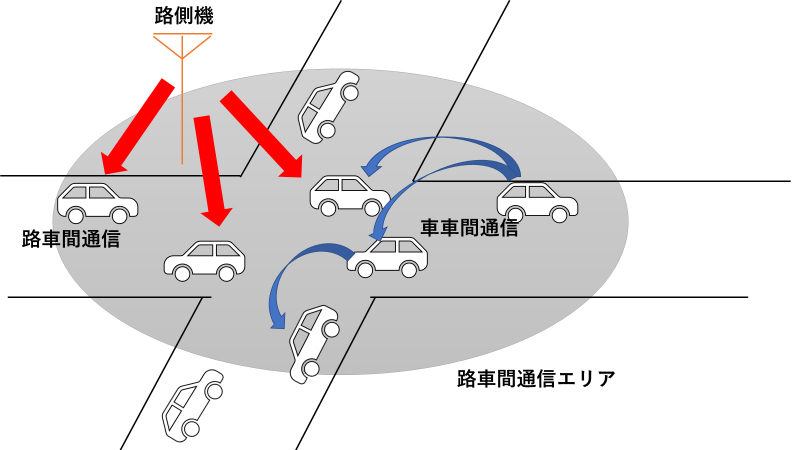
\includegraphics[width=10cm]{figures/2_2.png}
\caption{車車間通信と路車間通信}
\end{figure}

\section{関連研究}
継続して暴走行為を行う危険車両の検出を, 道路側のセンサに頼らず, 走行している車両間で行うためのVANETを用いた危険車両の検出手法が提案されている\cite{sample10}. 
 
既存研究では, 特にアドホック通信を用いたプロトコルの実現性を検証し, 周辺車両情報の収集技術の詳細に関しては述べていなかった. 以下, 前提条件として, 各車両(以下, 監視車両)は近隣車両(以下, 監視対象車両)の位置情報とID(ナンバープレートなど)を定期的に画像処理などの技術で取得できるものとする. この仮定の下, 各車両は周辺車両の車両IDと位置情報を取得すると, それらの車両IDと位置情報, 現在時刻, 自車両の位置情報, 警戒値を警戒情報としてブロードキャストする. 警戒値は監視対象車両の危険度を表す値であり, 初期値は0である. 警戒情報を後方から受信した車両は警戒情報を再ブロードキャストする. さらに, 受信した警戒情報中に記載された車両が近隣に存在し, 警戒情報中の位置情報と現在の位置情報が一定距離離れていれば, 速度を推定して(図\ref{fig:speed}), 速度超過をしているか否かを判定する. 警戒情報は図\ref{fig:detect}のように複数車両を介して前方車両へ伝搬する. 

この方式では, 車両密度が高い場合には高確率で違反車両の検知に成功している. しかし, 車両密度が増加すると隣接車両同士が同時に冗長なブロードキャストを行うため, パケット衝突やブロードキャストストーム\cite{sample11}などの問題が発生する. そのため, 制御パケット数の抑えながら高確率で危険車両の検知できる手法が必要である. 

\begin{figure}[H]
\centering
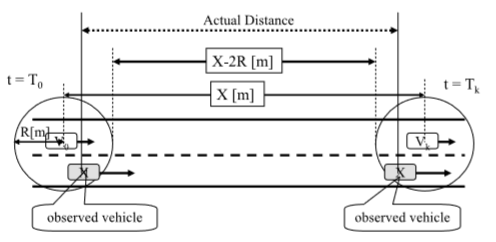
\includegraphics[width=12cm]{figures/2_4_1.png}
\caption{速度推定方法 ※井須 久美子, 藤木 健之, 梅津 高朗, 中 伊佐夫, 東野 輝夫, "車両の速度推定方法:車車間通信を用いた危険車両の検出車両の提案", 「情報処理学会論文誌」, 49, p213, 図1参照, 2008}
\label{fig:speed}
\end{figure}

\begin{figure}[H]
\centering
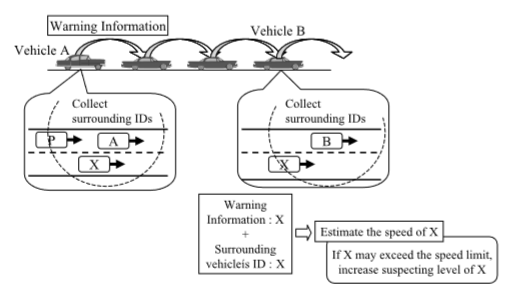
\includegraphics[width=12cm]{figures/2_4_2.png}
\caption{速度超過車両の検出方法 ※井須 久美子, 藤木 健之, 梅津 高朗, 中 伊佐夫, 東野 輝夫, "危険車両検出方法の概要:車車間通信を用いた危険車両の検出車両の提案", 「情報処理学会論文誌」, 49, p213, 図2参照, 2008}
\label{fig:detect}
\end{figure}


\chapter{VANETを用いた速度超過車両検出のためのブロードキャスト制御法}
\vspace{-5mm}
\section{概要}
既存のVANETを用いた速度超過車両の検知手法\cite{sample10}では, 車両密度が高い場合には高確率で違反車両の検知に成功している.しかし, 車両密度が増加すると違反車両検知のために送信される制御パケット数の増加が問題となる.

そこで本論文では, VANETを用いた速度超過車両検知を効率的に行うための速度推定手法と再ブロードキャスト制御アルゴリズムを提案する. 提案手法では, 周辺車両情報の収集のため, 各車両は車載カメラを用いて周辺車両のID(ナンバープレートなど)と位置情報を定期的に取得できることを前提とする. 車載カメラを用いて, 位置情報の取得方法の概要を図\ref{fig:image}に示す. 画像処理を用いて, 画像処理車両と監視対象車両との距離{\it L}を計測する. 画像処理車両の位置情報を$\bm{p}$とすると, 監視対象車両の位置情報$\bm{p}$ + $\dfrac{{\it L}}{||\textit{\textbf{p}}||}$ * $\bm{p}$となる. 画像処理を用いて, 車両間の距離測定誤差を向上させる研究は盛んに行われている\cite{sample15}\cite{sample16}. ステレオカメラを用いた場合と, 単眼カメラを用いた場合ともに距離測定は誤差数メートル以下に向上している.


\begin{figure}[H]
\centering
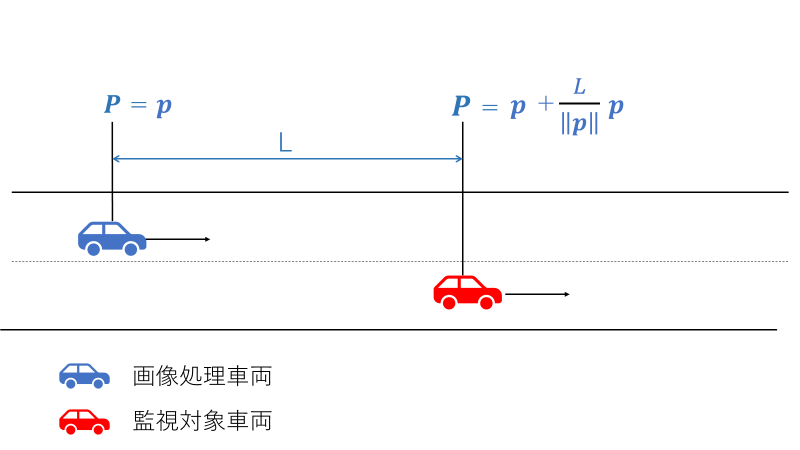
\includegraphics[width=12cm]{figures/3_1image.png}
\caption{位置情報の取得方法}
\label{fig:image}
\end{figure}

\section{速度推定手法}
速度推定は, 速度推定対象車両の決定と速度推定の2つのプロセスで構成される.速度推定の概要を図\ref{fig:Estimation}に示す.

\subsection{速度推定対象車両の決定}
各車両は車載カメラを用いて周辺車両のIDと位置情報を収集する. 他車両に追い越された場合, その車両を速度推定対象車両とみなし, その車両の警戒情報をブロードキャストする. 警戒情報を{\it W={id, $\bm{p}$, t, l, $\bm{p'}$, d}}で表す. {\it id} は速度推定対象車両の車両ID, $\bm{p}$は対象車両の位置情報, {\it t}は対象車両の位置を取得した時刻, {\it l}は警戒値, $\bm{p'}$はブロードキャストを行う車両の位置情報, $\bm{d}$はブロードキャストを行う車両の進行方向に関する情報である. 警戒値は対象車両の危険度を表す値であり, 初期値は0である. ブロードキャストを受け取った車両は,3.3節の手順に従い, $\bm{p'}$を自車両の位置情報に書き換えて再ブロードキャストを行う.

\begin{figure}[H]
\centering
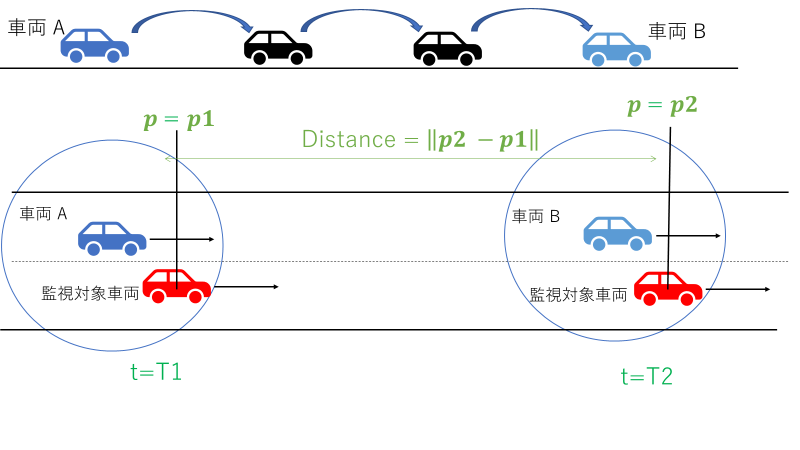
\includegraphics[width=12cm]{figures/3_2_1.png}
\caption{速度推定法}
\label{fig:Estimation}
\end{figure}

\subsection{速度推定}
各車両は速度推定対象車両を検知するか, 警戒情報を受信するまで待ち状態とする. 速度推定対象車両を検知した場合のアルゴリズムを図\ref{fig:detection}, 警戒情報を受信した場合のアルゴリズムが図\ref{fig:receive}に示す. また, 各アルゴリズムでは監視リストと転送リストを用いて処理を行う. ここで, 監視リストは, 後方から送られてきた警戒情報を保持するリストであり, 転送リストは前方へ送信すべき警戒情報を一時的に保持するリストである.監視リストと監視リストの例を表3.1に示す. まず, 速度推定対象車両を検知した場合のアルゴリズムについて述べる.

各車両は追い越し車両を検知すると, 監視リストに追い越し車両のIDが存在するかどうかを確認する. 監視リストにIDが存在しない場合, 即時に追い越し車両の警戒情報をブロードキャストする. 監視リストにIDが存在する場合, 監視リストに含まれる位置情報と現在取得した位置情報の距離の差{\it L}を求める. {\it L}が{\it Dmin}以上の場合のみ速度を推定する. 速度推定には式(3.1)を用いる. 式(3.1)において, {\it Vest}は推定速度, {\it R}は位置情報の最大誤差, 警戒情報が最初に発信された地 点(p)と時刻(t)をそれぞれ $\bm{Prec}$, {\it Trec}, 推測を行う地点と時刻をそれぞれ$\bm{Pcur}$, {\it Tcur}で表す. 提案手法では, 警戒値がある閾値を超えたときに, 警察に通報することを想定しているため, 誤検出を防ぐため推定速度は常に最小に設定している. 

% ボールドイタリック体 $\bm{p}$
 

\begin{equation}
Vest = \dfrac{||\textit{\textbf{Pcur - Prec}}|| - R}{Tcur – Trec}
\end{equation}
{\it Vest}が{\it Vmin}以上の時, その車両を速度超過車両とみなし, 監視リストに含まれる警戒値に1を足して, 警戒情報をブロードキャストする.

ここで, 定数{\it Dmin}は, 速度推定対象車両の, 速度を計測せず, 警戒情報を伝搬させるべき距離を表す. {\it Vmin}は速度超過車両とみなす最低速度である. また, 監視リストは一定時間ごとに古い情報は削除される. 

次に警戒情報を受信した場合のアルゴリズムについて述べる. 各車両は警戒情報を取得すると監視リストに取得したIDが存在するかを確認する. 存在しない場合は, 監視リストに取得した警戒情報を追加する. また, IDは監視リストに存在するが警戒値が上昇している場合, 監視リストの警戒値を更新する. 警戒情報を追加, または更新をした場合, 警戒情報は即時には再ブロードキャストをせず, 一時的に転送リストに保存する. その後, 3.3節の手順に従い, 再ブロードキャストを行うかパケットをドロップするかを選択する. 転送リストは3.3節の手順が終了すると即時に削除する. 
\begin{figure}[H]
\centering
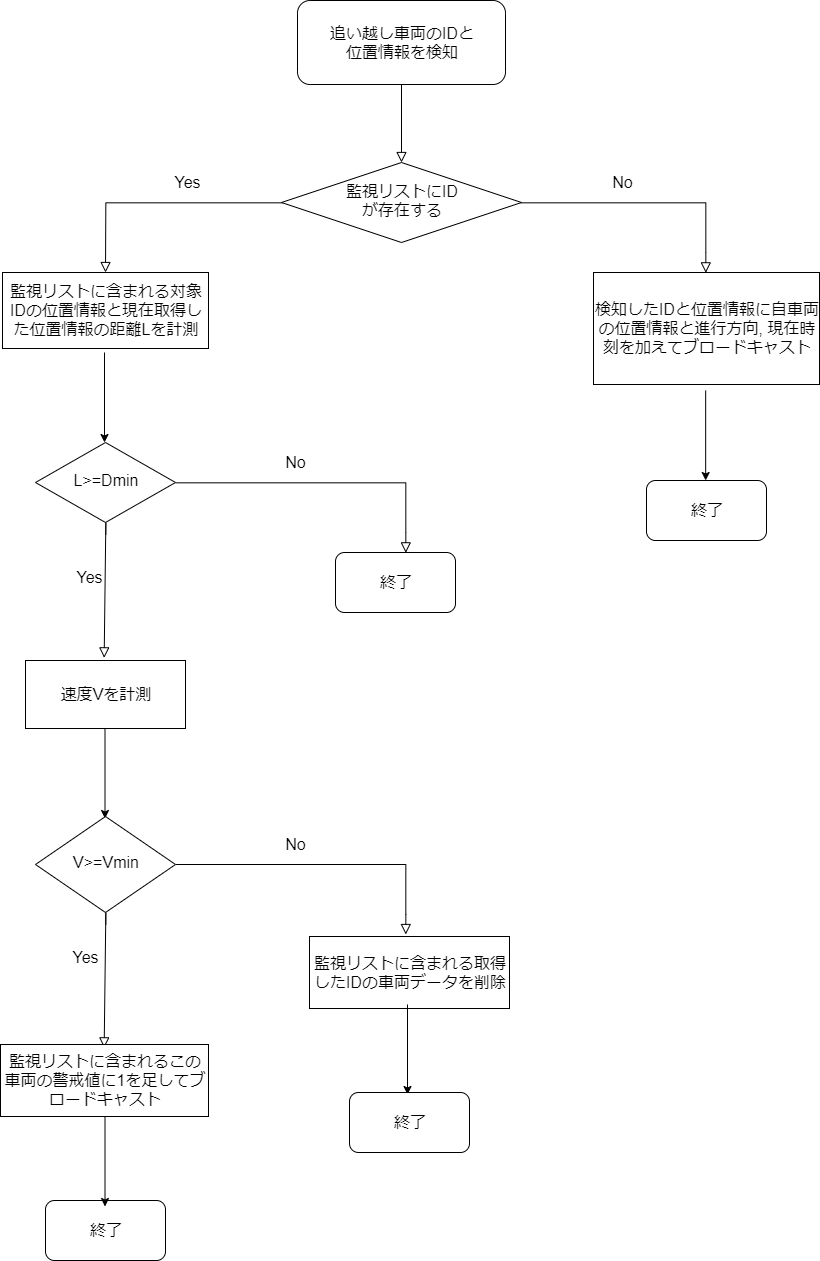
\includegraphics[width=12cm]{figures/detect3_2_2.png}
\caption{速度推定対象車両を検知した場合のアルゴリズム}
\label{fig:detection}
\end{figure}

\begin{figure}[H]
\centering
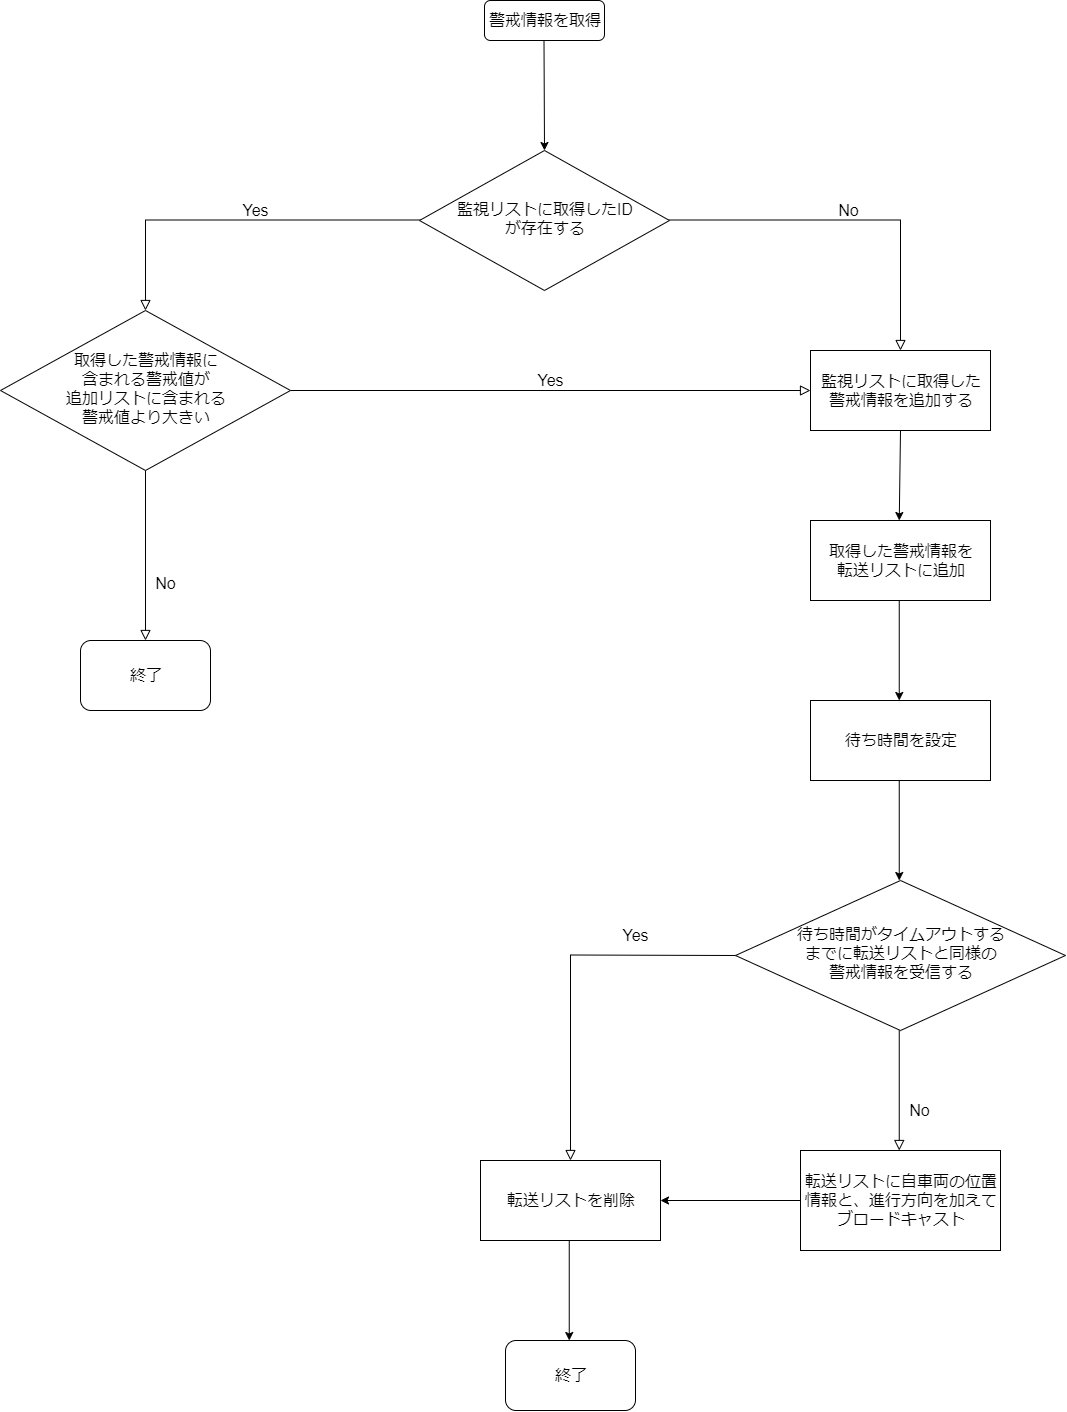
\includegraphics[width=12cm]{figures/receive3_2_2.png}
\caption{警戒情報を受信した場合のアルゴリズム}
\label{fig:receive}
\end{figure}


\begin{table}[H]
\caption{監視リスト 転送リストの例}
\centering
\begin{tabular}{|l|l|l|l|l}
\cline{1-4}
ID & 位置情報      & 取得時刻     & 警戒値 &  \\ \cline{1-4}
1  & (23,45)   & 11:45:35 & 1   &  \\ \cline{1-4}
4  & (456,678) & 12:34:45 & 0   &  \\ \cline{1-4}
68 & (32,6)    & 11:59:78 & 0   &  \\ \cline{1-4}
\end{tabular}
\end{table}


 
\section{再ブロードキャストの制御アルゴリズム}
既存手法では, 警戒情報を後方車両から受け取った車両が再ブロードキャストを行うため, 多数の車両が同一警戒情報を重複送信し無駄なブロードキャストが発生する. そこで本研究では, 再ブロードキャスト数を削減するアルゴリズムを提案する. 
 車両Aが送信した警戒情報を受け取った車両Bは, 即時に再ブロードキャストを行わず, 再ブロードキャストまで一定の待ち時間を設ける. 待ち時間の決定法の概要を図\ref{fig:waittime}に示す. 待ち時間{\it Wz}は式(3.2)で算出する. 
 
\begin{equation}
Wz = Z – \dfrac{Dcosθ}{ML} * Z
\end{equation}

{\it Z}は待ち時間の最大値, {\it D}は警戒情報を送信した車両と受信した車両の距離, {\it ML}は通信範囲の最大値, {\it θ}は警戒情報の送信車両の進行方向と, 送信車両と受信車両を結ぶ直線のなす角である.各車両は警戒情報を受信したとき(図\ref{fig:waittime}では車両Bのみ), 再ブロードキャストを行う警戒情報を一時的に転送リストに追加する. 待ち時間がタイムアウトするまでに, 転送リストに含まれる警戒情報と同一の警戒情報を受信したとき, 再ブロードキャストは行わず, 転送リストに含まれる警戒情報を削除する. このアルゴリズムによって一回の警戒情報を受け取る車両が複数存在した時, ブロードキャストをした車両から距離が離れた車両からタイムアウトが早くなり, 再ブロードキャストする確率が高くなる. その結果, 進行方向へ少ないブロードキャスト回数で伝搬することが可能になる. 

例えば, 待ち時間の最大値{\it Z}=1秒, 警戒情報を送信した車両と受信した車両の距離{\it D}が100m, 警戒情報の送信車両の進行方向と, 送信車両と受信車両を結ぶ直線のなす角{\it θ}が60°, 通信範囲の最大値{\it ML}が200mとすると, 待ち時間は以下のとおりである.
\begin{equation*}
W1=1 - \dfrac{100 × cos60}{200} × 1 = 0.75(秒)
\end{equation*}

\begin{figure}[H]
\centering
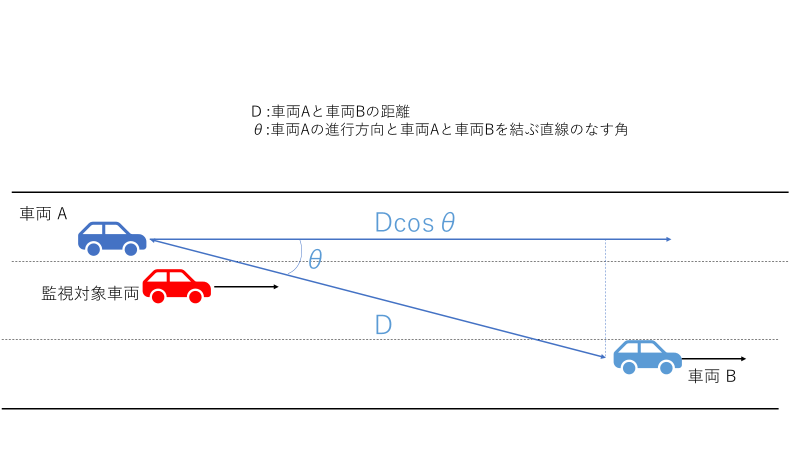
\includegraphics[width=12cm]{figures/3_3.png}
\caption{待ち時間の決定法}
\label{fig:waittime}
\end{figure}


\chapter{性能評価}
\vspace{-5mm}
\section{実験環境}
本シミュレーションでは, 片側3車線の高速道路を想定して, NS3(Network Simulator version3)\cite{sample12}を用いて評価した. また, 車線変更や追い越しなど現実的な車両のモビリティをNS3で再現することは難しいため, ノード(車両)のモビリティの作成には交通流シミュレーターであるSUMO(Simulation of Urban Mobiity)\cite{sample13}を用いた. シミュレーションパラメータを表4.1に示す. 4.3.1節でブロードキャスト数の比較を行うため, ホップ数の最大を8とした. 道路環境は, 4kmの3車線道路で, そのうち始点から500m地点のエリアを車両の生成エリアとする(図\ref{fig:roadmap}). 全車両は車両生成エリア内のランダムな位置に毎秒1〜10秒に1台ずつ(車両密度 80〜15台/4km)生成されて, 終点まで走行する. 車両の走行速度は制限速度と車両付近の車両の有無によってランダムに変化する. 制限速度は時速100kmとし, 速度超過車両の最高速度は120kmに設定した. また, 全車両数は110台, そのうち10台を速度超過車両とし, 通常車両は提案する検出プロトコルを実行するが, 速度超過車両については, 警戒情報の伝搬は行わないとした.  

\begin{table}[H]
\caption{シミュレーションパラメータ}
\centering
\begin{tabular}{|c|c|}
\hline
Network Simulator      & NS-3.29    \\ \hline
Mobility Simulator     & SUMO       \\ \hline
PHY layer              & 802.11p    \\ \hline
Transmission range(ML) & 200{[}m{]} \\ \hline
Image processing range & 40{[}m{]} \\ \hline
Road length            & 4{[}km{]}  \\ \hline
Number of cars         & 110        \\ \hline
Speed Limit       & 100{[}km/h{]}          \\ \hline
Limited Hopcount   & 8  \\ \hline
Dmin       & 800{[}m{]}          \\ \hline
Vmin       & 120{[}km/h{]}          \\ \hline
\end{tabular}
\end{table}


\begin{figure}[H]
\centering
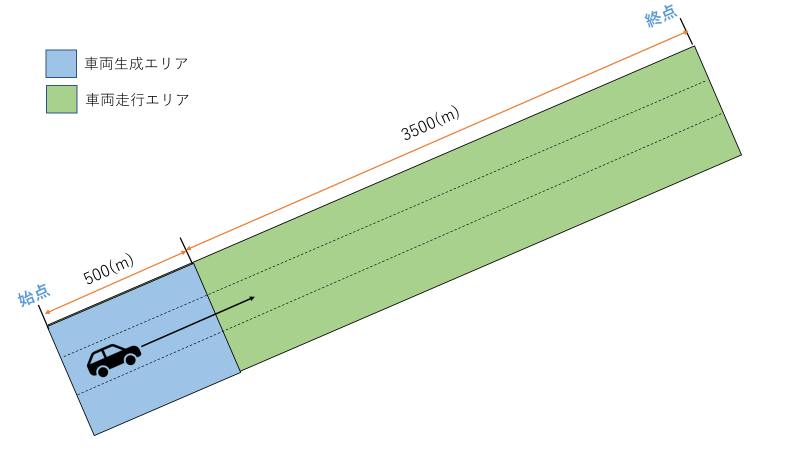
\includegraphics[width=12cm]{figures/4_1.png}
\caption{道路環境}
\label{fig:roadmap}
\end{figure}

\section{評価項目}
\subsubsection{速度超過車両の検出確率}
速度超過車両の検出確率{\it Pd}を式4.1で示す. 
\begin{equation}
Pd = \dfrac{検出した危険車両の台数}{走行している危険車両の台数}
\end{equation}
検出確率を用いて以下の, 1)ブロードキャスト数の比較, 2)再ブロードキャストの削減率, 3)位置情報の誤差の3つの指標から評価する. 

\subsubsection{1)ブロードキャスト数の比較}
本論文で提案した手法と, 既存研究の手法を比較する. 車両の発生間隔を変化させた場合のブロードキャスト数と検出確率の比較を行い評価する. 

\subsubsection{2)再ブロードキャストの削減率}
  3.3節で示した再ブロードキャスト制御法による, ネットワークトラヒック量の削減を再ブロードキャストの送信回数で評価する. 待ち時間の最大値{\it Z}を変化させたときの, 再ブロードキャストの送信回数の削減率{\it Rz}を算出する.  再ブロードキャストを制御しなかった場合の再ブロードキャスト数を{\it n1}, 再ブロードキャストを制御した場合の再ブロードキャスト数を{\it n2}とし, 再ブロードキャスト送信回数の削減率{\it Rz}は式4.2で算出する. 
\begin{equation}
Rz=(1-\dfrac{n2}{n1}) × 100
\end{equation}

例えば, 待ち時間の最大値Z=1, 再ブロードキャストを制御した場合の再ブロードキャストの送信回数が60回, 再ブロードキャストを制御しなかった場合の再ブロードキャストの送信回数を120回とすると, 再ブロードキャストの削減率は以下のとおりである. 
\begin{equation*}
R1=(1 - \dfrac{60}{120}) × 100 = 0.5(%)
\end{equation*}

この評価項目では, 待ち時間の最大値Zを変化させた場合の, 再ブロードキャストの削減率に与える影響と, 速度超過車両の検出確率に与える影響を考察する. 

\subsubsection{3)位置情報の誤差}
本研究では, 車両のIDと位置情報を車載のカメラによる画像処理によって, 取得することを前提としている. そのため, 画像処理による位置情報の精度の影響を評価しなければならない. そのため, 画像処理による位置情報の誤差を加えた場合の, 速度超過車両の検出確率の変化を評価する. 誤差の最大値を{\it R}としたとき, {\it R}から{\it -R}までの値をランダムに変化させたものを正規の座標に加えることによって, 位置情報の誤差を実装した. 誤差の最大値{\it R}を変化させたときの、速度超過車両の検出確率への影響を評価する.

\section{実験結果}
\subsection{ブロードキャスト数の比較}

図\ref{fig:brcount}は車両の発生間隔を変化させたときの提案手法, 既存手法それぞれのブロードキャストの回数を示している. 今回の実験では, 待ち時間の最大値{\it Z}は1秒, 誤差の最大値{\it R}は0(誤差なし)で行った. 提案手法は既存手法に比べて, ブロードキャスト回数を大幅に減らし, ネットワークトラヒックの削減ができていることがわかる. これは, 3.2節の速度推定手法により, 警戒情報のブロードキャストを追い越し車両のみとしたことと, 3.3節の再ブロードキャスト制御法により, 再ブロードキャストを行う車両を制御していることが原因だと考えられる. また, 既存手法, 提案手法ともに車両発生間隔が増加すると, ブロードキャスト数が減少していることがわかる. これは, 各車両の画像処理の範囲に存在する車両台数が減少していることと, 1度のブロードキャストの通信範囲内に存在する車両が減少し, パケットドロップとパケットロスが発生する割合が増加していることが原因と考えられる. 図\ref{fig:Pd}は車両の発生間隔を変化させたときの提案手法, 既存手法それぞれの速度超過車両の検出率を示している. ブロードキャストの回数を大幅に削減しても, 待ち時間の最大値{\it Z}が1秒の場合は, 速度超過車両の検出確率にほとんど影響が与えないことを示している. また, 車両発生間隔が増加するにつれて既存手法, 提案手法ともに検出確率が減少していることがわかる. これは, 警戒情報を前方に中継するときに, 中継車両が存在せずパケットロスしていることが原因だと考えられる.


\begin{figure}[H]
\centering
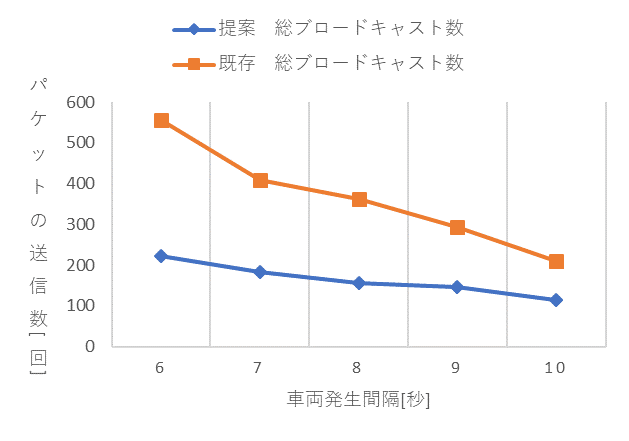
\includegraphics[width=14cm]{figures/4_3br.png}
\caption{ブロードキャスト回数の比較}
\label{fig:brcount}
\end{figure}

\begin{figure}[H]
\centering
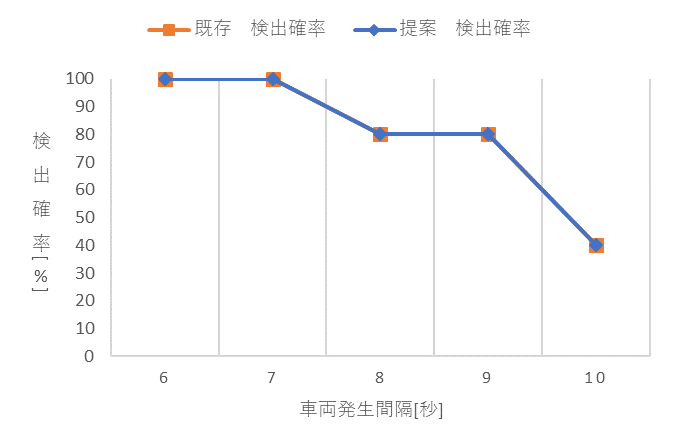
\includegraphics[width=14cm]{figures/4_3detect.png}
\caption{検出確率の比較}
\label{fig:Pd}
\end{figure}

\subsection{待ち時間の最大値における再ブロードキャスト削減率}
図\ref{fig:remove}は待ち時間の最大値Zを変化させたときの再ブロードキャストの削減率を示している。今回の実験では, 誤差の最大値{\it R}は0(誤差なし)で行った.削減率はZ=0.001秒から, Zの値が大きくなるにつれて, 削減率も大きくなっていることがわかる. また, Zが0.007秒以上になると再ブロードキャストの削減率は変化していないことがわかる. これは, Zが0.007秒以上になると警戒情報の再ブロードキャストを最適なノードだけが行っているからである. 実験結果から, 車両発生間隔が8秒(車両密度 17台/4km)のときにおいて, 再ブロードキャスト制御法を適用することで, 約20%のパケット送信を削減することを確認した. 車両密度が大きくなると, 一度のブロードキャストでパケットを受信する車両の台数が適用しない場合よりも増えるため, 再ブロードキャスト削減率は上昇することが予想される.

図\ref{fig:waitdetect}は待ち時間の最大値Zを変化させたときの, 検出確率を示している. 再ブロードキャストを制御しても, 速度超過車両の検出確率に影響がないことがわかる.

\begin{figure}[H]
\centering
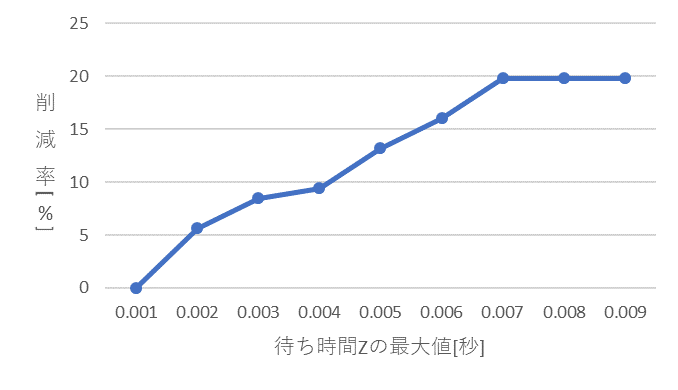
\includegraphics[width=14cm]{figures/4_3waittime.png}
\caption{再ブロードキャスト削減率}
\label{fig:remove}
\end{figure}

\begin{figure}[H]
\centering
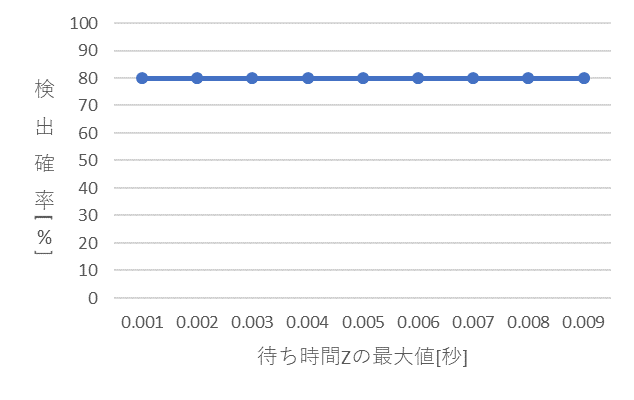
\includegraphics[width=14cm]{figures/4_3waitdetect.png}
\caption{待ち時間による検出確率への影響}
\label{fig:waitdetect}
\end{figure}

\subsection{位置情報の誤差が検出率に及ぼす影響}
図\ref{fig:error}は位置情報の誤差の最大値を変化させたときの, 検出確率を示している. また, 本実験ではDminの値は800mとした. 位置情報の誤差の最大値{\it R}が大きくなるにつれて, 検出確率が減少していることがわかる. 今回の実験で, 位置情報の誤差の最大値{\it R}が25m以上になると, 速度超過車両の検出確率が50\%以下まで低下することを確認した. 検出確率が低下してしまう原因は, 式(3.1)が示すように, 予め推測できる位置情報の誤差の最大値{\it R}を{\it Pcur - Prec}から引くことにより速度を低めに設定していることが原因だと考えられる. 

\begin{figure}[H]
\centering
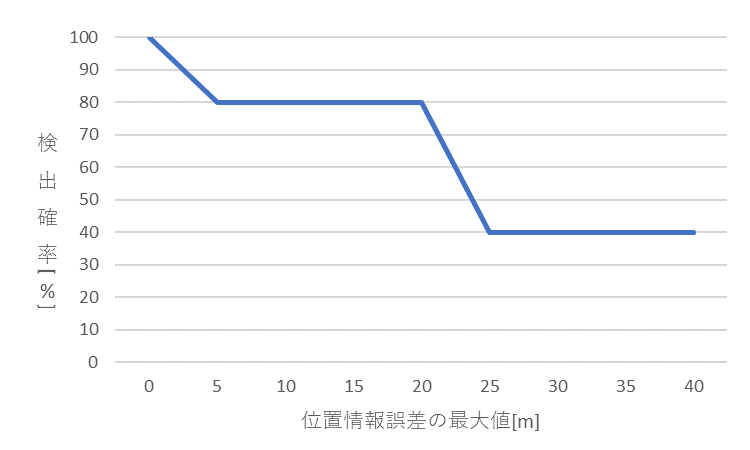
\includegraphics[width=14cm]{figures/4_3error.png}
\caption{検出確率の比較}
\label{fig:error}
\end{figure}


\chapter{結論}
本論文ではネットワークトラヒックの削減を目的とした新たなVANETを用いた速度推定手法と, 再ブロードキャスト制御法を提案した. 実験結果から, 総ブロードキャスト数の削減, 再ブロードキャスト削減率および速度超過車両の検出確率に与える影響を示した. また, 位置情報の誤差における速度超過車両の検出確率に与える影響を確認した. 第1章では本論文の構成内容や速度超過車両検出における既存のシステムの問題点を述べ, 第2章ではVANETについて既存のサービスや概要, VANETを用いた速度超過車両検出手法の既存研究について述べ, 第3章では本論文で提案したVANETを用いた速度超過車両検出のためのブロードキャストの制御方法について述べ, 第4章では提案手法の性能評価について述べた.

本論文ではネットワークトラヒックの削減を目的とした新たなVANETを用いた速度推定手法と, 再ブロードキャスト制御法を提案した.

今後の課題として, 道路の環境に応じた待ち時間の最大値{\it Z}を算出する手法の開発, 位置情報の誤差を修正するアルゴリズムの検討が必要である.

























\begin{comment}



\begin{equation}
酸素飽和度 = O_2Hb/(Hb+O_2Hb)
\end{equation}

\begin{enumerate}
\item 箇条書きの書き方\\
こんな感じで書きます
\item 箇条書きの書き方\\
増やすことも可能
\end{enumerate}

\begin{itemize}
\item 異なる箇条書き
\end{itemize}

図の入れ方
\begin{figure}[H]
\centering
\includegraphics[width=7cm]{figures/mig.eps}
\caption{図のキャプション}
\end{figure}

図を並べる入れかた
\begin{figure}[H]
\begin{minipage}{0.5\hsize}
\begin{center}

\includegraphics[width=7cm]{figures/Sample.png}
\end{center}
\caption{図のキャプション}
\end{minipage}
\begin{minipage}{0.5\hsize}
\begin{center}

\includegraphics[width=7cm]{figures/Sample.png}
\end{center}
\caption{図のキャプション}
\end{minipage}
\end{figure}

\begin{table}[H]
\caption{表の作り方}
\centering
\begin{tabular}{|l|c|c|c|} \hline
\multicolumn{2}{|l|}{} & \multicolumn{2}{|c|}{WiFi} \\ \cline{3-4}
\multicolumn{2}{|l|}{} & HTTPS & MQTT \\ \hline
receive & messages / hour & 3,628 & 263,314 \\ \cline{2-4}
 & \% battery / msg & 0.00095 & 0.00002 \\ \cline{2-4}
 & msgs(note losses) & 524 / 1024 & 1024 / 1024 \\ \hline
send & msg / hour & 5,229 & 23,184 \\ \cline{2-4}
 & \% battery / msg & 0.00104 & 0.00016 \\ \hline
\end{tabular}
\end{table}

\end{comment}


%参考文献の引用のしかた\cite{sample}.

\addcontentsline{toc}{chapter}{謝辞}
\chapter*{謝辞}
\sloppy
本論文では筆者が立命館大学情報理工学部情報コミュニケーション学科におい
て行なった「VANETを用いた速度超過車両検出のためのブロードキャスト制御法」の成果をまとめたものである.

本研究を遂行するにあたり,全過程を通じて懇切丁寧なる御指導,御鞭撻を賜わっ
た,立命館大学情報理工学部野口~拓教授に深甚なる感謝の意を表す.

立命館大学情報理工学部において,御指導,御教授を賜わった立命館大学情報理工学部Alberto Gallegos Ramonet特任助教, 前田~忠彦教授, 山本~寛准教授, 西村~俊和准教授, 瀧本~栄二助教を始め,各教員の方々に衷心より御礼申し上げる.

%本研究を遂行するにあたり,終始一貫して直接御指導戴いたネットワークシステム研究室の野口~拓講師に深甚なる感謝の意を表す.

ネットワークシステム研究室の諸兄には,日頃より多くの御助言,御協力戴き,種々の面でお世話になった.ここに深謝申し上げる.

ここに記して,以上の方々に深甚なる感謝の意を捧げる.
\addcontentsline{toc}{chapter}{参考文献}

%\newpage

\bibliographystyle{IEEEtran}
\bibliography{shuto}



%bibliographystyle{ フォーマット}
%bibliography{ビブファイルを指定}


\addcontentsline{toc}{chapter}{発表論文}
\chapter*{発表論文}
\small
[1]高橋 柊人, 野口 拓, 吉田 政望, ガジェゴス ラモネト アルベルト, "VANETを用いた速度超過車両検出のためのブロードキャスト制御法", 2020年電子情報通信学会総合大会(3月発表予定).

\end{document}
